%-------------------------------------------------------------------------------
%-------------------------------------------------------------------------------
%-------------------------------------------------------------------------------
\chapter{Images couleurs}
%-------------------------------------------------------------------------------
%-------------------------------------------------------------------------------
\thispagestyle{empty}
%--------------------------------------------------------------------------
%--------------------------------------------------------------------------
%--------------------------------------------------------------------------
% %--------------------------------------------------------------------------
% \section{Rappel : images monochromes}
% %--------------------------------------------------------------------------
% %--------------------------------------------------------------------------
% Une image est représentée dans un ordinateur sous la forme d'une mosaïque de petits carrés appelés \type{pixel}s\footnote{{\bf pic}ture {\bf el}ements}. Ces éléments sont codés dans un tableau dont les lignes et les colonnes correspondent aux positions dans l'image. On peut remarquer que cette décomposition en points est aussi celle qu'utilise notre œil qui reçoit la lumière dans des éléments appelés bâtonnets dans la rétine.

% \medskip

% Python possède une interface qui permet de traiter ces images sous la forme de tableaux gérés par le module \type{numpy}.

% Nous avons étudié en première année cette interface dans le cas des images monochrome qui sont en fait l'écriture d'une fonction de deux variables dont la valeur peut représenter la luminosité.
% %--------------------------------------------------------------------------
% \subsection*{Les outils}
% %--------------------------------------------------------------------------
% \begin{itemize}
% %--------------------------------------------------------------------------
% \item On doit charger les bibliothèques
% \begin{lstlisting}
% import numpy as np
% import matplotlib.pyplot as plt
% \end{lstlisting}
% %--------------------------------------------------------------------------
% \item Pour afficher une image que l'on a définie par une matrice on utilise \type{plt.imshow(image1)}.
% %--------------------------------------------------------------------------
% \item Par défaut les niveaux ne sont pas visualisés en niveau de gris. On peut ajouter l'échelle des couleurs employées avec \type{plt.colorbar()}
% %--------------------------------------------------------------------------
% \item On change l'échelle des couleurs avec le paramètre \type{cmap} (pour Color MAP)
  
%   \type{plt.imshow(image1,cmap='gray')}
% %--------------------------------------------------------------------------
% \item On peut voir les différentes échelles de couleurs à l'adresse
  
% \begin{verbatim}
%   http://matplotlib.org/examples/color/colormaps_reference.html
% \end{verbatim}
% %--------------------------------------------------------------------------
% \item Python peut effectuer un lissage utile pour améliorer le rendu. On peut l'activer avec le paramètre \type{interpolation}

% \type{plt.imshow(image1,cmap='gray',interpolation='bilinear')}
% %--------------------------------------------------------------------------
% \item On peut lire une image depuis la mémoire de masse :

% \type{img = plt.imread("/chemin/vers/l/image/mon\_image.png")}

% \type{img} est alors connu par python sous la forme d'un tableau numpy.
% %--------------------------------------------------------------------------
% \item Le nom complet du chemin est accessible dans le gestionnaire de fichiers (file browser) de Pyzo par un clic droit sur le nom du fichier. 

% On choisit "Copier le nom complet (chemin) du fichier".

% \newpage
% %--------------------------------------------------------------------------
% \item Il y a une image monochrome dans le module \type{scipy} :

% \begin{lstlisting}
% from scipy.misc import ascent

% a = ascent()
% plt.imshow(a,cmap='gray')
% \end{lstlisting}
% %--------------------------------------------------------------------------
% \item La taille d'une image est celle de la matrice associée que l'on obtient par \type{np.shape}.
% %--------------------------------------------------------------------------
% \end{itemize}
% % --------------------------------------------------------------------------
% % --------------------------------------------------------------------------
\section{Images en couleur}
%--------------------------------------------------------------------------
%--------------------------------------------------------------------------
\subsection{Première exploration}
%--------------------------------------------------------------------------
\type{scipy} contient une image en couleurs, un mignon raton-laveur.
\begin{lstlisting}
from scipy.misc import face

image1 = face()
\end{lstlisting}
%--------------------------------------------------------------------------
\begin{Exercise}\it Afficher l'image.

Quelle est sa taille ?
\end{Exercise}
%--------------------------------------------------------------------------
\begin{Answer}
\begin{lstlisting}
from scipy.misc import face

image1 = face()
plt.imshow(image1)
plt.show()

print(np.shape(image1))
\end{lstlisting}

\end{Answer}
On remarque que la matrice a trois dimensions.  

De plus l'image est tout de suite vue en "vraies couleur", \type{cmap} n'a aucun effet.
En effet les outils de \type{matplotlib} vont gérer le fait que l'image est composée de plusieurs couches.

\medskip

Le dossier public contient aussi une image aux couleurs plus marquées que celle que fournit \type{scipy} : \type{bouquet.png}.
%--------------------------------------------------------------------------
\begin{Exercise}\it Charger cette image en mémoire et l'afficher.
\end{Exercise}
%--------------------------------------------------------------------------
\begin{Answer}
\begin{lstlisting}
image2 = plt.imread("/home/ericd13/Travail/2016-2017/IC2/TP/TP1 Images/bouquet.png")

plt.imshow(image3)
plt.show()
\end{lstlisting}
\end{Answer}
%--------------------------------------------------------------------------
%--------------------------------------------------------------------------
\subsection{Séparation des couleurs}
%--------------------------------------------------------------------------
On a donc affaire à une structure de données à 3 dimensions : la hauteur, la largeur et la profondeur qui peut être 3\footnote{la profondeur peut être 4 quand on ajoute une composante de transparence.}. Dans l'interface \type{matplotlib} les valeurs de ce tableau sont le plus souvent des flottants compris entre 0 et 1 ou des entiers sur 8 bits, compris entre 0 et 255.

Pour voir l'effet de chaque couche nous allons créer des images qui n'utilisent qu'une des couches les deux autres étant mises à 0.

La première couche sera donc isolée par 
%--------------------------------------------------------------------------
\begin{lstlisting}
p, q, r = np.shape(image1)
couche0 = np.zeros((p, q, r))
for i in range(p):
    for j in range(q):
        couche0[i, j, 0] = image1[i, j, 0]
\end{lstlisting}
%--------------------------------------------------------------------------
On peut remplacer la double boucle par une extraction généralisée à une liste multiple : les trois dimensions sont séparées par des virgules et on sélectionne les portions par \type{a:b}. Si \type{a} est omis, il est remplacé par 0,  si \type{b} est omis, il est remplacé par la taille de la dimension.

%--------------------------------------------------------------------------
\begin{lstlisting}
p, q, r = np.shape(image1)
couche0 = np.zeros((p, q, r))
couche0[ : , : , 0] = image1[ : , : , 0]
\end{lstlisting}
%--------------------------------------------------------------------------

On peut aussi définir la matrice en annulant les couches à partir de l'image.

%--------------------------------------------------------------------------
\begin{lstlisting}
couche0 = np.copy(image1)
couche0[ : , : , 1] = 0
couche0[ : , : , 2] = 0
\end{lstlisting}
%-------------------------------------------------------------------------- 
On voit que \type{numpy} distribue ({\sc cast} en anglais) la valeur 0 à tous les points de l'extraction.
%--------------------------------------------------------------------------
\begin{Exercise}\it Déterminer de même les images ne contenant respectivement que la couche 1 et la couche 2 de l'image.
\end{Exercise}
%--------------------------------------------------------------------------
\begin{Answer}
\begin{lstlisting}
couche1 = np.copy(image1)
couche1[ : , : , 0] = 0
couche1[ : , : , 2] = 0

couche2 = np.copy(image1)
couche2[ : , : , 0] = 0
couche2[ : , : , 1] = 0
\end{lstlisting}
\end{Answer}
%--------------------------------------------------------------------------
On peut afficher plusieurs images en même temps :
%--------------------------------------------------------------------------
\begin{lstlisting}
plt.subplot(2, 2, 1) 
plt.imshow(image1)
plt.subplot(2, 2, 2) 
plt.imshow(couche0)
plt.subplot(2, 2, 3) 
plt.imshow(couche1)
plt.subplot(2, 2, 4) 
plt.imshow(couche2)
\end{lstlisting}
%--------------------------------------------------------------------------

On voit donc que les couleurs sont séparées en 3 composantes : rouge, vert et bleu.

On notera $(r,v,b)$ les composantes de la couleur d'un point elles sont obtenues par \type{image[i,j,:]}.
%--------------------------------------------------------------------------
\subsection{Création}
%--------------------------------------------------------------------------
\begin{Exercise}\it Définir une image de taille 300x300 nulle initialement dans laquelle on mettra les valeurs à 1 dans les partie décrites ci-après :
\begin{itemize}
\item le cercle de centre (135,124) de rayon 50 pour la première couche,
\item le cercle de centre (135,176) de rayon 50 pour la deuxième couche,
\item le cercle de centre (180,150) de rayon 50 pour la troisième couche.
\end{itemize}

\end{Exercise}
%--------------------------------------------------------------------------
\begin{Answer}
\begin{lstlisting}
image2 = np.zeros((300,300,3))
for i in range(300):
    for j in range(300):
        if (i -135)**2 + (j-124)**2 < 50**2:
            image2[i,j,0] = 1
        if (i -135)**2 + (j-176)**2 < 50**2:
            image2[i,j,1] = 1
        if (i -180)**2 + (j-150)**2 < 50**2:
            image2[i,j,2] = 1

plt.imshow(image2)
\end{lstlisting}
\end{Answer}
%--------------------------------------------------------------------------

On obtient une image classique d'illustration de la synthèse additive. 

Par exemple on voit que le jaune est obtenu en ajoutant le rouge et le vert.

Le résultat devrait ressembler à l'image \type{spots.png} qui se trouve dans le dossier public.

%--------------------------------------------------------------------------
\begin{Exercise}\it Créer le drapeau d'un pays de votre choix ; éviter les drapeaux compliqués comme celui du Royaume-Uni, préférer celui de la France, de la Belgique, de l'Italie, \dots
\end{Exercise}
%--------------------------------------------------------------------------
\begin{Answer}
\begin{lstlisting}
\end{lstlisting}
\end{Answer}
%--------------------------------------------------------------------------
%--------------------------------------------------------------------------
\section{Recollements d'images}
%--------------------------------------------------------------------------
%--------------------------------------------------------------------------
Le but de cette partie est d'assembler deux images en essayant de ne pas faire apparaître la liaison.
Si on applique à deux copies d'une même image on peut prolonger celle-ci ; c'est l'idée à la base du remplissage d'une surface par un motif.

Nous nous plaçons dans le cas particulier d'un placement côte-à-côte de deux images de même hauteur.

On note l1 la largeur de la première image et l2 la largeur de la seconde.

\begin{center}
\begin{tikzpicture}
\draw[pattern=north west lines, pattern color=blue] (0,0) rectangle (6,2);
\draw[pattern=north east lines, pattern color=red] (4,0) rectangle (9,2);
\draw[<->] (0,-0.2) -- node[below] {l1} (6, -0.2);
\draw[<->] (4,-0.4) -- node[below] {l2} (9, -0.4);
\draw[<->] (4,-0.6) -- node[below] {d} (6, -0.6);
\draw[<->] (-0.2,0) -- node[left] {h} (-0.2,2);
\end{tikzpicture}
\end{center}

Voici les images qui serviront dans les exemples.

\begin{center}
\includegraphics[scale=0.8]{IC_img1.png} 
\hskip 1cm
\includegraphics[scale=0.8]{IC_img2.png} 
\end{center}
%--------------------------------------------------------------------------
\begin{Exercise}\it 
Écrire une fonction \type{decoupe(img1,img2,d)} qui prend l1 - $\frac d 2$ pixels de gauche à img1 et l2-$\frac d 2$  pixels de droite de img2 et les associe : on découpe au milieu de la zone commune.
\end{Exercise}
%--------------------------------------------------------------------------
\begin{Answer}
\begin{lstlisting}
def decoupe(img1,img2,d):
    h,l1,n = img1.shape
    h,l2,n = img2.shape
    ll1 = l1 - d//2
    tout = np.zeros((h,l1+l2-d,n))
    tout[:,0:ll1,:] = img1[:,0:ll1,:]
    tout[:,ll1:,:] = img2[:,d-d//2:,:]
    return tout
\end{lstlisting}
\end{Answer}
%--------------------------------------------------------------------------
\begin{center}
\type{decoupe(img1,img2,100)} donne
\includegraphics[scale=0.8]{IC_reponseI1.png} 
\end{center}
%--------------------------------------------------------------------------
\begin{Exercise}\it 
Pour obtenir une transition moins brutale on va plutôt mélanger les deux images.
Écrire une fonction \type{melange(img1,img2,d)} qui calcule les pixel de la bande commune sous la forme $\displaystyle \type{img[x,y,k]} = \frac{\type{img1[x,y,k] + img2[x,y - l1 + d,k]}}2$.
Pourquoi divise-t-on par 2 ?
\end{Exercise}
%--------------------------------------------------------------------------
\begin{Answer}
\begin{lstlisting}
def melange(img1,img2,d):
    h,l1,n = img1.shape
    h,l2,n = img2.shape
    tout = np.zeros((h,l1+l2-d,n))
    tout[:,0:l1-d,:] = img1[:,0:l1-d,:]
    tout[:,l1:,:] = img2[:,d:,:]
    tout[:,l1-d:l1]=(img1[:,l1-d:,:]+img2[:,:d,:])/2
    return tout
\end{lstlisting}
\end{Answer}
%--------------------------------------------------------------------------
\begin{center}
\type{melange(img1,img2,100)} donne \includegraphics[scale=0.8]{IC_reponseI2.png} 
\end{center}
%--------------------------------------------------------------------------
\begin{Exercise}\it 
Le mélange ci-dessus manque encore de transition : on va mélanger progressivement.

Écrire une fonction \type{fondu(img1,img2,d)}  qui calcule les pixel de la bande commune sous la forme \type{img[x,y,k] = (1-t)img1[x,y,k] +   t *img2[x,y - l1 + d,k]} avec  $t = \frac {y-l1+d} d$ et $y$ compris entre l1 - d et l1.
\end{Exercise}
%--------------------------------------------------------------------------
\begin{Answer}
\begin{lstlisting}
def fondu(img1,img2,d):
    h,l1,n = img1.shape
    h,l2,n = img2.shape
    tout = np.zeros((h,l1+l2-d,n))
    tout[:,0:l1-d,:] = img1[:,0:l1-d,:]
    tout[:,l1:l1+l2-d,:] = img2[:,d:l2,:]
    for i in range(0,d):
        tout[:,l1-d+i,:] = (d-i)/d*img1[:,l1-d+i,:]+i/d*img2[:,i,:]
    return tout
\end{lstlisting}
\newpage
\end{Answer}
%--------------------------------------------------------------------------
\begin{center}
\type{fondu(img1,img2,100)} donne
\includegraphics[scale=0.8]{IC_reponseI3.png} 
\end{center}
%--------------------------------------------------------------------------
\newpage
%--------------------------------------------------------------------------
\section{Autre définition des couleurs}
%--------------------------------------------------------------------------
%--------------------------------------------------------------------------
Le modèle RVB employé ci-dessus est pratique pour le calcul des images mais rend difficile une modification cohérente des couleurs. On voudrait pouvoir augmenter/diminuer le caractère coloré des images (on parle de {\bf saturation}), augmenter/diminuer la luminosité et même transformer les couleurs ...

On a vu que les 3 composantes des couleurs décrivent un cube : $[0;1]^3$.

On peut remarquer que la diagonale du cube, de (0,0,0) à (1,1,1) représente les tons de gris et que sa direction semble indiquer la luminosité.
On va donc privilégier cette direction.

$$
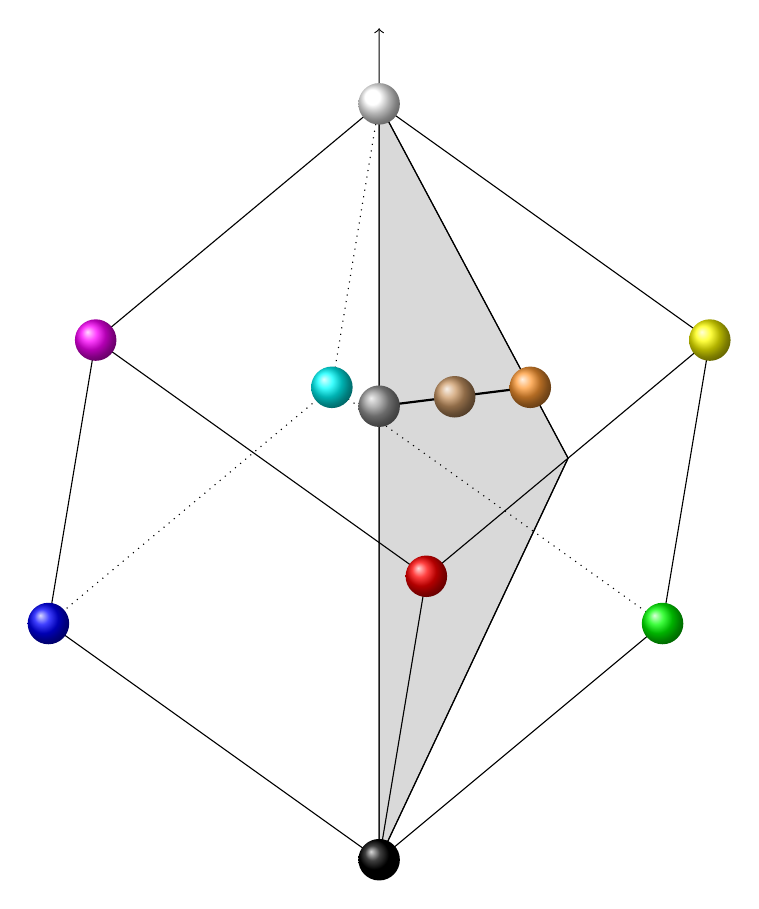
\begin{tikzpicture}[scale = 6,x={(0.1cm,0.6cm)},y={(0.6cm,0.5cm)},z={(-0.7cm,0.5cm)}]
\tikzset{boule/.style = {%draw,
                         shape          = circle,
                         text           = black,
                         inner sep      = 2pt,
                         outer sep      = 0pt,
                         minimum size   = 15 pt}}                
\definecolor{col1}{rgb}{0.8,0.6,0.4}
\definecolor{col2}{rgb}{0.6,0.6,0.6}
\definecolor{col3}{rgb}{1,0.6,0.2}
\definecolor{col4}{rgb}{1,0.5,0.0}
\coordinate (A0) at  (0,0,0);
\coordinate (A1) at  (1,0,0);
\coordinate (A2) at  (1,1,0);
\coordinate (A3) at  (0,1,0);
\coordinate (A4) at  (0,1,1);
\coordinate (A5) at  (0,0,1);
\coordinate (A6) at  (1,0,1);
\coordinate (A7) at  (1,1,1);
\coordinate (B1) at  (0.8,0.6,0.4);
\coordinate (B2) at  (0.6,0.6,0.6);
\coordinate (B3) at  (1,0.6,0.2);
\coordinate (B4) at  (1,0.5,0);
\draw[fill=gray!30] (A7) -- (B4) -- (A0) -- (A7);
\draw (A0) -- (A1) 
      (A0) -- (A3) 
      (A0) -- (A5) 
      (A6) -- (A7)
      (A2) -- (A7);
\draw[dotted]  (A4) -- (A7);
\draw[->] (0,0,0)-- (1.1,1.1,1.1);
\draw (A5) -- (A6) -- (A1) -- (A2) -- (A3);
\draw[dotted] (A3)  -- (A4) -- (A5);
\draw[thick] (B2)  -- (B1) -- (B3);
\draw(A7)  -- (B4) -- (A0);
\node[boule,ball color=black] at (A0){};
\node[boule,ball color=red] at (A1){};
\node[boule,ball color=green] at (A3){};
\node[boule,ball color=blue] at (A5){};
\node[boule,ball color=yellow] at (A2){};
\node[boule,ball color=magenta] at (A6){};
\node[boule,ball color=cyan] at (A4){};
\node[boule,ball color=white] at (A7){};
\node[boule,ball color=col1] at (B1){};
\node[boule,ball color=col2] at (B2){};
\node[boule,ball color=col3] at (B3){};
\end{tikzpicture}
$$

Nous allons choisir une représentation qui ressemble aux représentation HSV et HSL\footnote{Voir \type{https://en.wikipedia.org/wiki/HSL\_and\_HSV}} mais dont les calculs sont simplifiés. Pour cela nous utiliserons les coordonnées cylindrique avec un axe porté par $(1,1,1)$. L'angle est déterminé de telle manière que les couleurs rouges, les points (r,0,0) ou (1,s,s), définissent un angle nul.

On commence par définir une nouvelle base orthonormée $(\vec u_1, \vec u_2, \vec u_3)$ dont le troisième vecteur dirige l'axe. Le choix de la couleur rouge comme angle initial impose que le plan engendré par $\vec u_1$ et $\vec u_3$ contienne le rouge, c'est-à-dire le vecteur $(1,0,0)$.

On aboutit à $\displaystyle \vec u_1 = \frac 1{\sqrt 6}\begin{pmatrix} 2\\ -1\\ -1\\ \end{pmatrix}$ $\displaystyle \vec u_2 = \frac 1{\sqrt 2}\begin{pmatrix} 0\\ 1\\ -1\\ \end{pmatrix}$ et $\displaystyle \vec u_3 = \frac 1{\sqrt 3}\begin{pmatrix} 1\\ 1\\ 1\\ \end{pmatrix}$.

Une couleur de composantes $(r, v, b)$ sera donc définie par les nouvelles coordonnées $(X, Y, Z)$ avec 
$\displaystyle \begin{pmatrix} r\\ v\\ b\\ \end{pmatrix}
=X  \vec u_1+Y \vec u_2+ Z\vec u_3$ 
d'où $\displaystyle r = \frac {2X}{\sqrt 6} + \frac Z{\sqrt 3}$, $\displaystyle v = -\frac {X}{\sqrt 6} + \frac Y{\sqrt 2}+\frac Z{\sqrt 3}$ et  $\displaystyle b = -\frac {X}{\sqrt 6} - \frac Y{\sqrt 2}+\frac Z{\sqrt 3}$


On pose alors $X =S\cos(H)$ et $Y=S\sin(\varphi)$ en coordonnées polaires donc $S=\sqrt{X^2+Y^2}$ et l'angle $H$ est l'argument du complexe $X+iY$ que l'on peut calculer par une fonction \type{numpy} : \type{H = np.arctan2(Y,X)}.

On pose aussi $\displaystyle I = \frac Z{\sqrt 3} =\frac {r+v+b}{3}$ pour obtenir un réel dans $[0;1]$.
\begin{itemize}
\item $H $ (pour \type{\bf hue}, teinte en anglais) indique la teinte. 
\item $S$ est l'éloignement du gris, c'est une mesure de la saturation en couleur.
 
\item On a vu que $I$ mesurait la luminosité.
\end{itemize}

La saturation n'atteint pas la valeur 1 : voici les couleurs qui ont une luminosité $I = 0,6$, cela correspond à la section du cube par un plan perpendiculaire à l'axe de gris.

%-------------------------------------------------------------------------------
\begin{minipage}{0.50\textwidth}
\vspace{0pt}
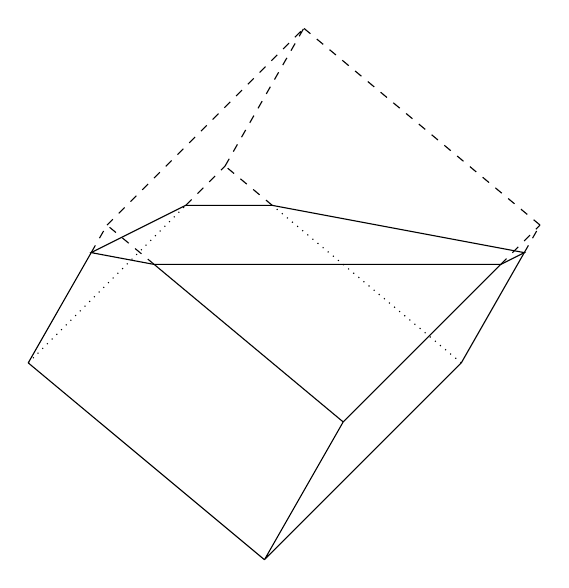
\begin{tikzpicture}[scale = 5,x={(0.2cm,0.35cm)},y={(0.5cm,0.5cm)},z={(-0.6cm,0.5cm)}]
\coordinate (A0) at  (0,0,0);
\coordinate (A1) at  (1,0,0);
\coordinate (A2) at  (1,1,0);
\coordinate (A3) at  (0,1,0);
\coordinate (A4) at  (0,1,1);
\coordinate (A5) at  (0,0,1);
\coordinate (A6) at  (1,0,1);
\coordinate (A7) at  (1,1,1);
\coordinate (H1) at (1, 0.8, 0);
\coordinate (H2) at (0.8, 1, 0);
\coordinate (H3) at (0, 1, 0.8);
\coordinate (H4) at (0, 0.8, 1);
\coordinate (H5) at (0.8, 0, 1);
\coordinate (H6) at (1, 0, 0.8);
\draw (A0) -- (A1) 
      (A0) -- (A3) 
      (A0) -- (A5) 
      (A1) -- (H1)
      (A1) -- (H6)
      (A3) -- (H2)
      (A5) -- (H5);
\draw[dotted]
      (A3) -- (H3)
      (A5) -- (H4);
\draw[dashed]
      (H1) -- (A2)
      (H2) -- (A2)
      (H3) -- (A4)
      (H4) -- (A4)
      (H5) -- (A6)
      (H6) -- (A6)
      (A2) -- (A7)
      (A4) -- (A7)
      (A6) -- (A7);
\draw (H1) -- (H2) -- (H3) -- (H4) -- (H5) -- (H6) -- (H1);
\end{tikzpicture}
\end{minipage}
%-------------------------------------------------------------------------------
\begin{minipage}{0.5\textwidth}
\vspace{0pt}
\includegraphics[scale=0.6]{IC_luminosite_0_6} 
\end{minipage}
%-------------------------------------------------------------------------------
On remarque toutes les valeurs s'obtiennent à l'aide de fonctions simples donc on pourra les calculer globalement en appliquant les fonctions aux tableaux.

On définira les matrices des couleurs par \type{R = image[:,:,0]}, de même pour \type{V} et \type{B}.

La matrice des $X$ se calcule alors par \type{X = (R + V + B)/np.sqrt(3)}.

%--------------------------------------------------------------------------
\begin{Exercise}\it Écrire une fonction \type{HSI(image)} qui renvoie les matrices des 3 composantes des couleurs des points.
\end{Exercise}
%--------------------------------------------------------------------------
\begin{Answer}
\begin{lstlisting}
def HSI(image):
    R = image[:,:,0]
    V = image[:,:,1]
    B = image[:,:,2]
    X = (2*R-V-B)/np.sqrt(6)
    Y = (V-B)/np.sqrt(2)
    I = (R+V+B)/3
    H = np.arctan2(Y,X)
    S = np.sqrt(X*X+Y*Y)
    return (H,S,I)
\end{lstlisting}
\end{Answer}
%--------------------------------------------------------------------------
%--------------------------------------------------------------------------
\begin{Exercise}\it Écrire une fonction \type{faireImage(H,S,I)} qui renvoie l'image reconstituée à partir des composantes $(H,S,I)$ des couleurs.

\end{Exercise}
%--------------------------------------------------------------------------
\begin{Answer}
\begin{lstlisting}
def faireImage(H,S,I):
    X = S*np.cos(H)
    Y = S*np.sin(H)
    haut, larg = np.shape(H)
    image = np.zeros((haut,larg,3))
    image[:,:,0] = 2*X/np.sqrt(6) + I
    image[:,:,1] = -X/np.sqrt(6) + Y/np.sqrt(2) + I
    image[:,:,2] = -X/np.sqrt(6) - Y/np.sqrt(2) + I
    return np.clip(image,0,1)
\end{lstlisting}
\end{Answer}
%--------------------------------------------------------------------------
\medskip
Des composantes transformées peuvent donner des valeurs de r, g ou b qui ne sont pas dans $[0;1]$. On tronquera les valeurs pour qu'elles restent entre 0 et 1 à l'aide de la fonction \type{np.clip(x,0,1)} qui renvoie 0 pour $x < 0$, $x$ pour $0\le x \le 1$ et 1 pour $x> 1$.
%--------------------------------------------------------------------------
\begin{Exercise}\it Transformer les images (raton-laveur ou bouquet). On pourra
\begin{itemize}
\item modifier la teinte en ajoutant une constante à H,
\item modifier la luminosité en multipliant I par une constante positive,
\item modifier la saturation en multipliant I par une constante positive.
\end{itemize}

Dans le cas des multiplications on expérimentera avec un facteur supérieur à 1 et un facteur inférieur à 1.
\end{Exercise}
%--------------------------------------------------------------------------
\begin{Answer}
\end{Answer}
%--------------------------------------------------------------------------
%--------------------------------------------------------------------------
